\section{Description et analyse d'une entreprise atypique: Probespoke}
\subsection{ProBespoke une entreprise innovante}

\paragraph{}
Probespoke a été fondé en 2012. Il s'agissait tout d'abord de réunir les différentes usines textiles de Bangkok.
Une plateforme informatique commune devais permettre la distribution des commandes venant d'Europe et d'Amérique du Nord.
\paragraph{}
\begin{wrapfigure}[12]{o}{8cm}
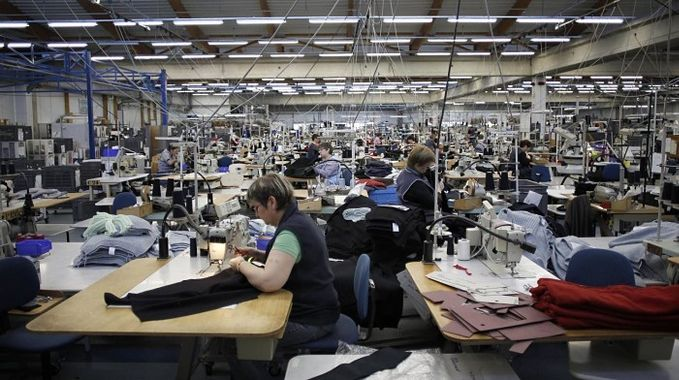
\includegraphics[width=8cm]{image/textile.jpg}
\caption{Une usine quelque part}
\end{wrapfigure}
Mais une différence de point vus à fait éclater le projet. Un des fondateurs, Christophe Saska décida de reprendre le projet sous une forme différente. Il agit comme un trader entre des tailleurs principalement européeen et américain et les usines thailandaises. En effet la fabrication d'une pièce sur mesure est décomposé sur plusieurs poste sur la chaine de fabrication. Une équipe s'occupe que des manches, une autre des poches, et ainsi de suite. Ces équipes ont besoin d'être formées par des maitres tailleurs expérimenté afin de correspondre aux attentes qualités du client. Cette charge de travail est difficile à supporter pour des tailleurs occidentaux peut habitués aux façon de travailler en Thailande. Du côté des ateliers thailandais, cet intermédiare leur permet de ne pas avoir à s'occuper du démarchage des clients. Il s'agit donc d'une opportunité pour tout le monde.
